%!TEX root = informe.tex
\chapter{Análisis de Ciclo de Vida: fabricación}
% Manual Euroadoquín. Documentos de Malaka.

\section{Obtención de datos}
Los datos de partida que se han utilizado en este análisis han sido proporcionados por Malaka de Prefabricados. La figura \ref{fig:diagrama_de_flujo} muestra las entradas al sistema, así como los procesos que ocurren durante la fabricación —que serán explicados en las siguientes secciones— y la salida del sistema.

\begin{figure}[!htb]
\centering
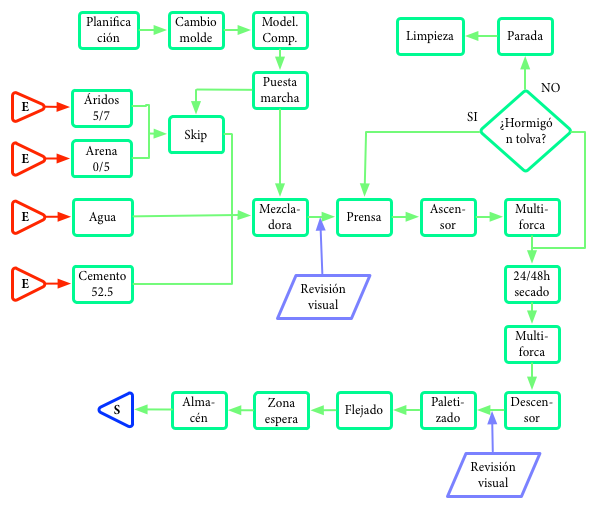
\includegraphics[width=15cm]{diagrama.png}
\caption{Diagrama de flujo de la fabricación de adoquines.}
\label{fig:diagrama_de_flujo}
\end{figure}

En primer lugar es necesario señalar que el modelo de adoquín ``Holanda 6'', cuya hoja de datos técnicos aparece en el Apéndice \ref{apend:catalogo}, es el que mayor demanda de fabricación tiene en la empresa, por lo que se ha dispuesto de mayor número de datos.

Cada bandeja fabricada supone exactamente 0.5 \si{m^2} de adoquines modelo ``Holanda 6''. Como se ha tomado como Unidad Funcional 1 \si{m^2} de adoquín, los cálculos se han realizado para 2 bandejas. Cada adoquín mide 200x100x60 \si{mm} y pesa 3 \si{kg}. Como cada bandeja está formada por 25 adoquines, y son necesarias 2 bandejas para tener 1 \si{m^2}, se tiene un total de 50 adoquines/\si{m^2} (ecuación \ref{eq:masa}). De esta forma:

\begin{gather}
200 mm \times 100 mm \times 25 ud/bandeja \times 2 bandeja = 1 m^2\\
3 kg/ud \times 50 ud/m^2 = 150 kg/m^2 \text{ de masa para adoquín}\label{eq:masa}
\end{gather}

Como es necesario disponer de 150 \si{kg/m^2} de masa para adoquín, se aplican los porcentajes de materias primas sobre la fórmula base para adoquín ``Holanda 6'' para obtener las masas de cada materia prima reflejadas en la tabla \ref{desglosemateriasprimas}.

\begin{table}[!htb]
\centering
\begin{tabular}{lcccc}
\toprule
\multicolumn{5}{c}{Consumo de materias primas por \si{m^2} de adoquín fabricado}\\
\midrule
Materia prima & \% Fórmula & Masa (\si{kg}) & Proced. & Dist. (\si{km})\\
\midrule
Árido tipo 5/7 & 37.75 & 56.63 & Alh. Torre & 8\\
Arena tipo 0/5 & 47.16 & 70.74 & Alh. Torre & 8\\
Cemento Portland 52.5N & 10.06 & 15.09 & Málaga-El Palo & 30\\
Agua & 5.03 & 7.54 & Red & -\\
\bottomrule
\end{tabular}
\caption{Desglose de materias primas por \si{m^2} de adoquín fabricado.}
\label{desglosemateriasprimas}
\end{table}

En el Apéndice \ref{apend:catalogo} también se especifica un diagrama de Gantt de los procesos para una simulación realizada para fabricar 1 \si{m^2} de adoquín, además de los consumos energéticos desglosados.

\section{Modelado de los procesos}
\subsection{Cemento}
El cemento se transporta a granel en camiones con tanques a presión hasta la fábrica. Allí se almacena en silos provistos de compresores que descargan el material desde el tanque hasta su interior. El compresor es alimentado por electricidad mediante una toma de corriente conectada a la red eléctrica. La descarga del silo es únicamente por gravedad con válvulas dosificadoras de control de caudal (ver tabla \ref{modeladodelcemento}).

Las unidades para el modelado del camión (lorry) vienen expresadas en \si{kg\times km}, mientras que el uso del silo se proporciona en \si{m^3}, dada una densidad media del cemento Portland de 1250 \si{kg/m3} \cite{website:ecoinvent}.

\begin{gather}
15.09 kg \times 30 km = 453 kg\times km\\
15,09 kg / 1250 kg/m^3 = 0.0121 m^3
\end{gather}

El mix eléctrico se obtiene del consumo del compresor del silo proporcional a una cantidad de 15.09 \si{kg}, si la potencia del compresor son 30kW, velocidad de carga del silo es 35 \si{\tonne/h} para un tiempo de llenado de 35 minutos.

\begin{gather}
30 kW \times 1 h \times \frac{35 min}{60 min} = 17.5 kWh = 63 MJ \text{ para 20 toneladas}\\
35 t/h \times \frac{35 min}{60 min} = 20 t \text{ de cemento con el silo cargado}\\
15.09 kg \times \frac{63 MJ}{20 t} = 4.79 kJ
\end{gather}

\begin{table}[!htb]
\centering
\begin{tabular}{p{8cm}rc}
\toprule
\multicolumn{3}{c}{Cemento Portland CEM I 52.5Z gris}\\
\midrule
Materiales/Ensamblajes & Cantidad & Unidad\\
\midrule
Portland cement, strength class Z 52.5, at plant/CH U & 15.09 & \si{kg}\\
\midrule
Procesos & Cantidad & Unidad\\
\midrule
Transport, lorry 16-32t, EURO4/RER U & 453 & \si{kg*km}\\
Tower silo, plastic/CH/I U & 0.0121 & \si{m^3}\\
Electricity mix 2013/ES U & 4.79 & \si{kJ}\\
\bottomrule
\end{tabular}
\caption{Modelado del cemento.}
\label{modeladodelcemento}
\end{table}

\subsection{Arena y áridos}
Las arenas y áridos se transportan hasta la planta de fabricación mediante camiones. Actualmente los áridos y la arena ya no se apilan a bajo techados en las explanadas adyacentes a las plantas, sino que el propio transporte rellena las tolvas de forma automática.

El tipo de arena que se utiliza en la planta es 0/5 —granulometría en milímetros de las partículas que forman la arena— no está directamente disponible en SimaPro. En su lugar, se ha optado por tomar el material ``Sand 0/2'' (Arena tipo 0/2), que además de pertenecer a la clasificación general de arena —de 0 a 5 \si{mm}—, la descripción de SimaPro indica que puede utilizarse como árido natural estándar en la industria de la construcción (ver tabla \ref{modeladodelaarena}).

\begin{quote}
Technical purpose of product or process: Standard mineral product used as natural aggregates in the construction industry according to the applied technology.
\end{quote}

Las unidades para el modelado del camión (lorry) vienen expresadas en \si{kg\times km}.

\begin{equation}
70.74 kg \times 8 km = 566 kg\times km
\end{equation}

\begin{table}[!htb]
\centering
\begin{tabular}{p{8cm}rc}
\toprule
\multicolumn{3}{c}{Arena tipo 0/5}\\
\midrule
Materiales/Ensamblajes & Cantidad & Unidad\\
\midrule
Sand 0/2, wet and dry quarry, production mix, at plant, undried/RER S & 70.74 & \si{kg}\\
\midrule
Procesos & Cantidad & Unidad\\
\midrule
Transport, lorry 16-32t, EURO4/RER U & 566 & \si{kg*km}\\
\bottomrule
\end{tabular}
\caption{Modelado de la arena.}
\label{modeladodelaarena}
\end{table}

Los áridos utilizados para producir adoquines puede incluir arena, gravilla y piedra de machaqueo si se pretende obtener un producto de peso normal. Si se desea que el adoquín sea más ligero —entre un 20 y un 45 \%— sin mermar sus propiedades estructurales se utilizan materiales como pizarra, arcilla, escoria de altos hornos y cenizas de carbón según su disponibilidad y coste.

El tipo de árido utilizado en planta es de granulometría 5/7 —en milímetros—, catalogado como gravilla. No está directamente disponible en SimaPro, por lo que en su lugar, se ha optado por tomar el material ``Gravel, crushed'' (gravilla de machaqueo) (tabla \ref{modeladodearido}).

Las unidades para el modelado del camión (lorry) vienen expresadas en \si{kg\times km}.

\begin{equation}
56.63 kg \times 8 km = 566 kg\times km
\end{equation}

\begin{table}[!htb]
\centering
\begin{tabular}{p{8cm}rc}
\toprule
\multicolumn{3}{c}{Árido tipo 5/7}\\
\midrule
Materiales/Ensamblajes & Cantidad & Unidad\\
\midrule
Gravel, crushed, at mine/CH U & 56.63 & \si{kg}\\
\midrule
Procesos & Cantidad & Unidad\\
\midrule
Transport, lorry 16-32t, EURO4/RER U & 453 & \si{kg*km}\\
\bottomrule
\end{tabular}
\caption{Modelado del árido.}
\label{modeladodearido}
\end{table}


\subsection{Agua}
La mayoría de las plantas tienen una fuente de agua municipal (\textit{tap water}) que proporciona potable perfectamente válida para el uso en la fabricación de hormigón (ver tabla \ref{modeladodelagua}).

\begin{table}[!htb]
\centering
\begin{tabular}{p{8cm}rc}
\toprule
\multicolumn{3}{c}{Agua}\\
\midrule
Materiales/Ensamblajes & Cantidad & Unidad\\
\midrule
Tap water, at user/RER U & 7.54 & \si{kg}\\
\bottomrule
\end{tabular}
\caption{Modelado del agua.}
\label{modeladodelagua}
\end{table}

\subsection{Cintas transportadoras de áridos y cemento}

Las tolvas descargan la cantidad programada de materia prima sobre dos cintas transportadoras —una para áridos y arena, otra para cemento— con básculas de pesaje incorporadas que se comunican con el sistema de control y cortan el flujo de descarga.

La cinta de áridos descarga sobre un skip que eleva los materiales hasta una mezcladora. La cinta de cemento descarga directamente sobre la mezcladora.

Las distancias están medidas sobre planos (Apéndice \ref{apend:planos}), y los consumos se han obtenido de los ensayos en fábrica a partir de la potencia de la cinta transportadora y el tiempo de funcionamiento (Potencia=Energía/Tiempo).

\begin{table}[!htb]
\centering
\begin{tabular}{p{8cm}rc}
\toprule
\multicolumn{3}{c}{Cinta transportadora para arena y áridos}\\
\midrule
Materiales/combustibles & Cantidad & Unidad\\
\midrule
Conveyor belt, at plant/RER/I U & 14.6 & \si{m}\\
\midrule
Electricidad/calor & Cantidad & Unidad\\
\midrule
Electricity mix 2013/ES U & 0.1827 & \si{MJ}\\
\bottomrule
\end{tabular}
\caption{Modelado de la cinta transportadora para arena y áridos.}
\label{modeladodecintaarena}
\end{table}

\begin{table}[!htb]
\centering
\begin{tabular}{p{8cm}rc}
\toprule
\multicolumn{3}{c}{Cinta transportadora para cemento}\\
\midrule
Materiales/combustibles & Cantidad & Unidad\\
\midrule
Conveyor belt, at plant/RER/I U & 7.3 & \si{m}\\
\midrule
Electricidad/calor & Cantidad & Unidad\\
\midrule
Electricity mix 2013/ES U & 0.0975 & \si{MJ}\\
\bottomrule
\end{tabular}
\caption{Modelado de la cinta transportadora para cemento.}
\label{modeladodecintacemento}
\end{table}

\subsection{Skip y mezcladora}

Previamente al añadido del agua se produce un ciclo de mezclado en seco. Para asegurar la consistencia del lote el agua es generalmente añadido mediante un sistema electrónico de control que dosifica el caudal. En el caso de que haya otros aditivos, tales como acelerantes o colorantes, es en este momento cuando se incorporan a la mezcla. Cuando se termina de añadir el agua se produce el mezclado creando hormigón fresco. El hormigón sale de la mezcladora mediante una cinta transportadora que contiene otra báscula de pesaje y se dirige hacia la tolva de hormigón que se encuentra en lo alto de la prensa, donde es dosificado en los moldes para adoquines. Los moldes tienen una longevidad muy alta —aproximadamente un millón de ciclos de prensado— y su durabilidad depende de las propiedades abrasivas de los áridos utilizados.

El molde se compone de dos partes: la parte donde se inyecta el hormigón (hembra) y la parte que se coloca encima para dar forma (macho). La prensa tiene incorporado un carro alimentador encargado de proporcionar la parte hembra. Se inyecta el hormigón en el molde hembra, el molde macho baja con la prensa y el hormigón es compactado y cimentado usando un sistema combinado de presión y vibración. Cada molde puede producir 25 adoquines de 200x100x60\si{\milli\meter}, lo que proporciona a una superficie adoquinada de 0.5\si{\square\meter}. Los adoquines son moldeados de una sola pieza y extraidos del molde inmediatamente después de la vibro-compresión sobre una bandeja de madera.

La bandeja con las piezas frescas es trasladada sobre un transportador de rodillos hasta un ascensor. Este ascensor tiene diez alturas, de forma que cada vez que recibe una bandeja con adoquines frescos, la bandeja anterior sube una altura y monta la siguiente.

El ascensor se encarga de alimentar un carro multiforca de diez alturas. Cuando las diez alturas está ocupadas se cargan en un carro multiforca automatizado que transporta las piezas hasta un secadero.

Las piezas permanecen en el secadero curándose a temperatura ambiente entre 24 y 48 horas.

Una vez transcurrido el tiempo de curado, los adoquines están secos y listos para ser recogidos por otro carro multiforca automatizado que recoge las bandejas y las lleva a un descensor.

El descensor coloca las bandejas con los adoquines secos en un transportador de rodillos.

El transportador de rodillos lleva las bandejas hasta una paletizadora para hacer bloques de hasta cinco alturas.

La paletizadora impulsa el pallet hasta la flejadora que aplica varias lazadas de flejes para evitar que los adoquines se desprendan del conjunto.

La flejadora descansa los conjuntos paletizados sobre un un transportador de rodillos para ser posteriormente llevados a almacén.

Finalmente, un torito transporta cada conjunto de adoquines a la zona de almacenaje.


\subsection{Dosificación}
\subsection{Amasado}
\subsection{Vibrocompresión}
\subsection{Curado}
\subsection{Embalaje y almacenamiento}
\subsection{Suministro}
\subsection{Recepción}


\begin{table}[!htb]
\centering
\begin{tabular}{p{8cm}rc}
\toprule
\multicolumn{3}{c}{Ascensor}\\
\midrule
\multicolumn{2}{c}{Materiales/combustibles}\\
\cmidrule(r){1-2}
Descripción & Cantidad & Unidad\\
\midrule
Steel, low-alloyed, at plant/RER U & 320 & \si{kg}\\
\midrule
\multicolumn{2}{c}{Electricidad/calor}\\
\cmidrule(r){1-2}
Descripción & Cantidad & Unidad\\
\midrule
Electricity mix 2013/ES U & 0.126 & \si{MJ}\\
\bottomrule
\end{tabular}
\caption{Modelado del ascensor.}
\label{modeladodelascensor}
\end{table}

\begin{table}[!htb]
\centering
\begin{tabular}{p{8cm}rc}
\toprule
\multicolumn{3}{c}{Descensor}\\
\midrule
\multicolumn{2}{c}{Materiales/combustibles}\\
\cmidrule(r){1-2}
Descripción & Cantidad & Unidad\\
\midrule
Steel, low-alloyed, at plant/RER U & 320 & \si{kg}\\
\midrule
\multicolumn{2}{c}{Electricidad/calor}\\
\cmidrule(r){1-2}
Descripción & Cantidad & Unidad\\
\midrule
Electricity mix 2013/ES U & 0.126 & \si{MJ}\\
\bottomrule
\end{tabular}
\caption{Modelado del descensor.}
\label{modeladodeldescensor}
\end{table}

\begin{table}[!htb]
\centering
\begin{tabular}{p{8cm}rc}
\toprule
\multicolumn{3}{c}{Cepillado, volteado y lubricado de bandejas}\\
\midrule
\multicolumn{2}{c}{Materiales/combustibles}\\
\cmidrule(r){1-2}
Descripción & Cantidad & Unidad\\
\midrule
Lubricating oil, at plant/RER U & 0.0001 & \si{kg}\\
Polyurethane, flexible foam, at plant/RER U & 1 & \si{kg}\\
Nylon 66, glass-filled, at plant/RER U & 4 & \si{kg}\\
Fleece, polyethylene, at plant/RER U & 0.6 & \si{kg}\\
\midrule
\multicolumn{2}{c}{Electricidad/calor}\\
\cmidrule(r){1-2}
Descripción & Cantidad & Unidad\\
\midrule
Electricity mix 2013/ES U & 0.0018 & \si{MJ}\\
\bottomrule
\end{tabular}
\caption{Modelado del cepillado, volteado y lubricado de bandejas.}
\label{modeladodelcepillado}
\end{table}





\begin{table}[!htb]
\centering
\begin{tabular}{p{8cm}rc}
\toprule
\multicolumn{3}{c}{Cinta transportadora para hormigón}\\
\midrule
\multicolumn{2}{c}{Materiales/combustibles}\\
\cmidrule(r){1-2}
Descripción & Cantidad & Unidad\\
\midrule
Conveyor belt, at plant/RER/I U & 12.1 & \si{m}\\
\midrule
\multicolumn{2}{c}{Electricidad/calor}\\
\cmidrule(r){1-2}
Descripción & Cantidad & Unidad\\
\midrule
Electricity mix 2013/ES U & 0.088 & \si{MJ}\\
\bottomrule
\end{tabular}
\caption{Modelado de la cinta transportadora para hormigón.}
\label{modeladodecintahormigon}
\end{table}

\begin{table}[!htb]
\centering
\begin{tabular}{p{8cm}rc}
\toprule
\multicolumn{3}{c}{Cinta transportadora para piezas frescas}\\
\midrule
\multicolumn{2}{c}{Materiales/combustibles}\\
\cmidrule(r){1-2}
Descripción & Cantidad & Unidad\\
\midrule
Conveyor belt, at plant/RER/I U & 6.8 & \si{m}\\
\midrule
\multicolumn{2}{c}{Electricidad/calor}\\
\cmidrule(r){1-2}
Descripción & Cantidad & Unidad\\
\midrule
Electricity mix 2013/ES U & 0.077 & \si{MJ}\\
\bottomrule
\end{tabular}
\caption{Modelado de la cinta transportadora para piezas frescas.}
\label{modeladodecintapiezas}
\end{table}

\begin{table}[!htb]
\centering
\begin{tabular}{p{8cm}rc}
\toprule
\multicolumn{3}{c}{Control informatizado}\\
\midrule
\multicolumn{2}{c}{Materiales/combustibles}\\
\cmidrule(r){1-2}
Descripción & Cantidad & Unidad\\
\midrule
Desktop computer, without screen, at plant/GLO U & 2 & p\\
Keyboard, standard version, at plant/GLO U & 2 & p\\
LCD flat screen, 17 inches, at plant/GLO U & 2 & p\\
Mouse device, optical, with cable, at plant/GLO U & 2 & p\\
Network access devices, internet, at user/CH/I U & 2 & p\\
Router, IP network, at server/CH/I U & 1 & p\\
Power supply unit, at plant/CN U & 2 & p\\
\midrule
\multicolumn{2}{c}{Electricidad/calor}\\
\cmidrule(r){1-2}
Descripción & Cantidad & Unidad\\
\midrule
Electricity mix 2013/ES U & 0.486 & \si{MJ}\\
\bottomrule
\end{tabular}
\caption{Modelado del control informatizado.}
\label{modeladodecontrol}
\end{table}


% DOSIDIFICADORES
% TORITO

\begin{table}[!htb]
\centering
\begin{tabular}{p{8cm}rc}
\toprule
\multicolumn{3}{c}{Flejado y paletizado}\\
\midrule
\multicolumn{2}{c}{Materiales/combustibles}\\
\cmidrule(r){1-2}
Descripción & Cantidad & Unidad\\
\midrule
Packing, clay products/CH U & 150 & \si{kg}\\
\midrule
\multicolumn{2}{c}{Electricidad/calor}\\
\cmidrule(r){1-2}
Descripción & Cantidad & Unidad\\
\midrule
Electricity mix 2013/ES U & 0.065 & \si{MJ}\\
\bottomrule
\end{tabular}
\caption{Modelado del flejado.}
\label{modeladodelflejado}
\end{table}

\begin{table}[!htb]
\centering
\begin{tabular}{p{8cm}rc}
\toprule
\multicolumn{3}{c}{Iluminación}\\
\midrule
\multicolumn{2}{c}{Materiales/combustibles}\\
\cmidrule(r){1-2}
Descripción & Cantidad & Unidad\\
\midrule
CFL Bulb 40W & 60 & p\\
\multicolumn{2}{c}{Desglose para 1 p. CFL Bulb 40W}\\
\cmidrule(r){1-2}
Aluminium alloy, AlMg3, at plant/RER U & 7.09 & \si{g}\\
Oriented polypropylene film E & 4.25 & \si{g}\\
Iron-nickel-chromium alloy, at plant/RER U & 6.27 & \si{g}\\
Copper wire, technology mix, consumption mix, at plant, cross section 1 \si{mm^2} EU-15 S & 4.25 & \si{g}\\
41 Plastics basic, virgin, EU27 & 1.42 & \si{g}\\
Integrated circuit, IC, logic type, at plant/GLO U & 1.42 & \si{g}\\
\midrule
\multicolumn{2}{c}{Electricidad/calor}\\
\cmidrule(r){1-2}
Descripción & Cantidad & Unidad\\
\midrule
Electricity mix 2013/ES U & 0.972 & \si{MJ}\\
\bottomrule
\end{tabular}
\caption{Modelado de la iluminación.}
\label{modeladodeiluminacion}
\end{table}

\begin{table}[!htb]
\centering
\begin{tabular}{p{8cm}rc}
\toprule
\multicolumn{3}{c}{Multiforca}\\
\midrule
\multicolumn{2}{c}{Materiales/combustibles}\\
\cmidrule(r){1-2}
Descripción & Cantidad & Unidad\\
\midrule
Steel, low-alloyed, at plant/RER U & 930 & \si{kg}\\
\midrule
\multicolumn{2}{c}{Electricidad/calor}\\
\cmidrule(r){1-2}
Descripción & Cantidad & Unidad\\
\midrule
Electricity mix 2013/ES U & 0.516 & \si{MJ}\\
\bottomrule
\end{tabular}
\caption{Modelado de la multiforca.}
\label{modeladomultiforca}
\end{table}

\begin{table}[!htb]
\centering
\begin{tabular}{p{8cm}rc}
\toprule
\multicolumn{3}{c}{Prensado}\\
\midrule
\multicolumn{2}{c}{Materiales/combustibles}\\
\cmidrule(r){1-2}
Descripción & Cantidad & Unidad\\
\midrule
Industrial machine, heavy, unspecified, at plant/RER/I U & 1380 & \si{kg}\\
\midrule
\multicolumn{2}{c}{Electricidad/calor}\\
\cmidrule(r){1-2}
Descripción & Cantidad & Unidad\\
\midrule
Electricity mix 2013/ES U & 0.437 & \si{MJ}\\
\bottomrule
\end{tabular}
\caption{Modelado del prensado.}
\label{modeladoprensado}
\end{table}


\begin{table}[!htb]
\centering
\begin{tabular}{p{8cm}rc}
\toprule
\multicolumn{3}{c}{Skip y mezcladora}\\
\midrule
\multicolumn{2}{c}{Materiales/combustibles}\\
\cmidrule(r){1-2}
Descripción & Cantidad & Unidad\\
\midrule
Plaster mixing/CH U & 150 & \si{kg}\\
\midrule
\multicolumn{2}{c}{Electricidad/calor}\\
\cmidrule(r){1-2}
Descripción & Cantidad & Unidad\\
\midrule
Electricity mix 2013/ES U & 1.71 & \si{MJ}\\
\bottomrule
\end{tabular}
\caption{Modelado del skip y la mezcladora.}
\label{modeladoskip}
\end{table}

\begin{table}[!htb]
\centering
\begin{tabular}{p{8cm}rc}
\toprule
\multicolumn{3}{c}{Tolva de hormigón}\\
\midrule
\multicolumn{2}{c}{Materiales/combustibles}\\
\cmidrule(r){1-2}
Descripción & Cantidad & Unidad\\
\midrule
Steel, low-alloyed, at plant/RER U & 470 & \si{kg}\\
\midrule
\multicolumn{2}{c}{Electricidad/calor}\\
\cmidrule(r){1-2}
Descripción & Cantidad & Unidad\\
\midrule
Electricity mix 2013/ES U & 0.0161 & \si{MJ}\\
\bottomrule
\end{tabular}
\caption{Modelado de la tolva de hormigón.}
\label{modeladotolva}
\end{table}




\begin{table}[!htb]
\centering
\begin{tabular}{p{8cm}rc}
\toprule
\multicolumn{3}{c}{Transporte de bandejas hasta paletizadora}\\
\midrule
\multicolumn{2}{c}{Materiales/combustibles}\\
\cmidrule(r){1-2}
Descripción & Cantidad & Unidad\\
\midrule
Roller conveyor, at plant/RER/I U & 6.88 & \si{m}\\
\midrule
\multicolumn{2}{c}{Electricidad/calor}\\
\cmidrule(r){1-2}
Descripción & Cantidad & Unidad\\
\midrule
Electricity mix 2013/ES U & 0.021 & \si{MJ}\\
\bottomrule
\end{tabular}
\caption{Modelado del transporte de bandejas hasta paletizadora.}
\label{modeladobandejaspalet}
\end{table}

\begin{table}[!htb]
\centering
\begin{tabular}{p{8cm}rc}
\toprule
\multicolumn{3}{c}{Transporte de pallets flejados hasta zona de recogida}\\
\midrule
\multicolumn{2}{c}{Materiales/combustibles}\\
\cmidrule(r){1-2}
Descripción & Cantidad & Unidad\\
\midrule
Roller conveyor, at plant/RER/I U & 39.1 & \si{m}\\
\midrule
\multicolumn{2}{c}{Electricidad/calor}\\
\cmidrule(r){1-2}
Descripción & Cantidad & Unidad\\
\midrule
Electricity mix 2013/ES U & 0.0315 & \si{MJ}\\
\bottomrule
\end{tabular}
\caption{Modelado del transporte de pallets flejados hasta zona de recogida.}
\label{modeladopalletsrecogida}
\end{table}

\begin{table}[!htb]
\centering
\begin{tabular}{p{8cm}rc}
\toprule
\multicolumn{3}{c}{Transporte de pallets hasta flejadora}\\
\midrule
\multicolumn{2}{c}{Materiales/combustibles}\\
\cmidrule(r){1-2}
Descripción & Cantidad & Unidad\\
\midrule
Roller conveyor, at plant/RER/I U & 3.1 & \si{m}\\
\midrule
\multicolumn{2}{c}{Electricidad/calor}\\
\cmidrule(r){1-2}
Descripción & Cantidad & Unidad\\
\midrule
Electricity mix 2013/ES U & 0.021 & \si{MJ}\\
\bottomrule
\end{tabular}
\caption{Modelado del transporte de pallets hasta flejadora.}
\label{modeladopalletsflejadora}
\end{table}

\begin{table}[!htb]
\centering
\begin{tabular}{p{8cm}rc}
\toprule
\multicolumn{3}{c}{Roller conveyor, at plant/RER/I U}\\
\midrule
\multicolumn{2}{c}{Materiales/combustibles}\\
\cmidrule(r){1-2}
Descripción & Cantidad & Unidad\\
\midrule
Concrete, sole plate and foundation, at plant/CH U & 0.01 & \si{m^3}\\
Section bar rolling, steel/RER U & 500 & \si{kg}\\
Steel, low-alloyed, at plant/RER U & 530 & \si{kg}\\
Transport, lorry >16t, fleet average/RER U & 55.5 & \si{\tonne*\km}\\
Wire drawing, steel/RER U & 29.6 & \si{kg}\\
\bottomrule
\end{tabular}
\caption{Modelado de 1 metro de cinta de rodillos.}
\label{modeladoroller}
\end{table}













